\documentclass[letterpaper,12pt]{article}
\usepackage{geometry}
\usepackage{multicol}
\usepackage{lipsum}
\usepackage{changepage}
\usepackage{graphicx}
\graphicspath{  }
\usepackage{booktabs}
\usepackage{cite}
\usepackage{float}
\usepackage{hyperref}
\usepackage[font={small}]{caption}
\usepackage[english]{babel}
\usepackage{fancyhdr}
\usepackage[T1]{fontenc}

\graphicspath {{figures/}}

\setlength{\headheight}{15pt}

\pagestyle{fancy}
\fancyhf{}
\lhead{\textbf{Version:} 1.0  \textbf{Revision:} 04/30/18}
\rhead{\thepage}
\lfoot{Caleb Lindsey}
\rfoot{\textit{Mu2e: University of Minnesota}}

\renewcommand{\footrulewidth}{1pt}




\begin{document}
\begin{titlepage}
	\centering
	
\includegraphics[width=0.5\textwidth]{mu2e_logo_oval.png}\par\vspace{2cm}
	{\scshape\LARGE Procedure for Generating Straw Barcodes\par}
	\vspace{3cm}
	{\Large Caleb Lindsey\par}
	\vspace{3cm}
	{\large University of Minnesota\par}
 	\vspace{.5cm}
	{\large April 30, 2018\par}
	% Bottom of the page
	\vfill
	{linds551@umn.edu\par}
\end{titlepage}

\clearpage
\setcounter{page}{2}

\newenvironment{myitemize} %adjust item spacing in lists to make smaller
{ \begin{itemize}
    \setlength{\itemsep}{4pt}
    \setlength{\parskip}{0pt}
    \setlength{\parsep}{0pt}     }
{ \end{itemize}                  } 

\section{Goal}
In order to effectively manage the straws, each will be given an ID number and a barcode.  With these the straws can be easily identified and their progress through each stage of production can be managed.  This SOP will cover how to generate barcodes for a pallet of 24 straws.
%%Insert your text here...same follows below%%

\section{Equipment}

\begin{multicols}{2}
\begin{myitemize}
	\item Printer
    \item Computer with barcode generator software
    \item Printer paper
    \item Scissors
    \item Clear tape
\end{myitemize}
\end{multicols}






\section{Procedure}
 Barcode generation should be done on the computer in the back room of 464.  Going through this procedure once will only generate 12 straws, so for a full 24 straw pallet, run through this twice.
\begin{enumerate}
	\item Locate the "barcodes.xlsx" file on the desktop and open it.  The file contents should look like figure \ref{fig:bar} but have different straw indexes.
    
    \begin{figure} [h]
		\centering
		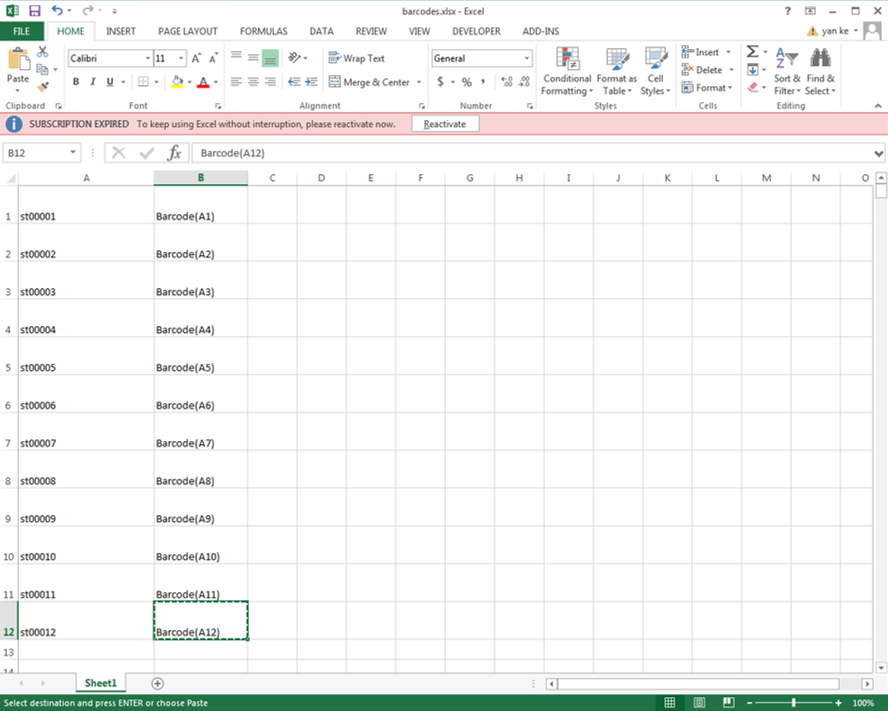
\includegraphics[width=.75\textwidth]{barcodesSOP.png}
		\caption{Contents of "barcodes.xlsx".  Change the values in column "A" to match the straws on the pallet.  Then save and close the file.  Make sure this file is on the desktop NEXT TO the barcode generator program.}
		\label{fig:bar}
	\end{figure}
    
    \item Do not touch column "B". Replace the names of the straws in column A to the ones on your pallet.  Then save and close the document.
    \item Double click on the "Barcode Generator" icon on the desktop to open the user interface.  Navigate through the top tabs until you are under "Excel Barcode Label Maker".  The window should look like figure \ref{fig:dummy}.  Make sure the barcode file edited in the previous step is the one next to the barcode generator icon on the desktop.
    \item In the Barcode generator, set the barcode format to "Code 39" and set the barcode width to "minimum width".  Make sure all other settings match figure \ref{fig:dummy}.  Click "Create Barcode Label -$>$ Excel".
    \item A read-only excel spreadsheet should open.  Save this file as a pdf and then print.  The printer is the Brother8510DN located just below the computer.
     \item Cut out the barcodes into one long strip and tape them on the end of a pallet so that the lowest barcode index corresponds to the bottom of the pallet.
     \item To fill a full pallet, repeat this process and add the next twelve barcodes to the remaining unlabeled straws.
    \end{enumerate}
   
\section{Cleanup}
\begin{enumerate}
	\item Recycle paper scraps and put scissors and tape away in their respective drawers.
    \item Make sure there is still paper in the printer for the next barcode generation.  Refill the printer if it is empty.  If you do not know where paper is, ask a manager.

\end{enumerate}

 \begin{figure} [h]
		\centering
		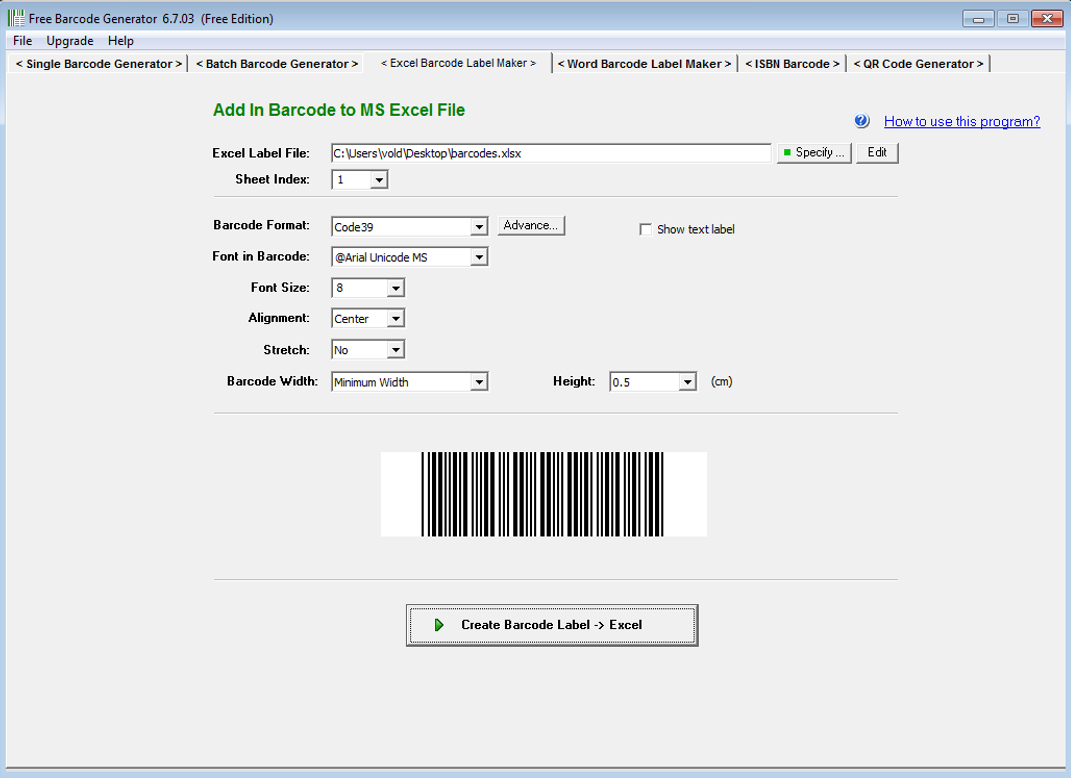
\includegraphics[width=.75\textwidth]{BarcodeGeneratorSOP.png}
		\caption{The Barcode generator is located on the desktop.  When creating barcodes, set the format to 39 and the width to "Minimum".}
		\label{fig:dummy}
	\end{figure}
	


\section{Troubleshooting}

\begin{itemize}
	\item {\bf Problem:} The printer is not printing
		\begin{adjustwidth}{1cm}{}
		{\bf Solution:} Make sure the printer is on and has paper and ink. Recycle the connection by turning of the printer and turning it back on, or disconnecting it from the computer.  If this does not work ask a manager. 
		\end{adjustwidth}
	\item {\bf Problem:} The "barcodes.xlsx" file is missing or modified.
		\begin{adjustwidth}{1cm}{}
		{\bf Solution:} The file can be easily recreated by recreating figure \ref{fig:bar}.  Type the desired straw indexes in column "A" and type "Barcode(A\#)" in each "B" column. 
		\end{adjustwidth}
	

\end{itemize}



\end{document}